% ---------------------------------------------------------------------------
% Author guideline and sample document for EG publication using LaTeX2e input
% D.Fellner, v1.13, Jul 31, 2008

\documentclass{egpubl}
\usepackage{eurovis2018}
\Full_EuroVis
% --- for  Annual CONFERENCE
% \ConferenceSubmission   % uncomment for Conference submission
%\ConferencePaper        % uncomment for (final) Conference Paper
% \STAR                   % uncomment for STAR contribution
% \Tutorial               % uncomment for Tutorial contribution
% \ShortPresentation      % uncomment for (final) Short Conference Presentation
% \Areas                  % uncomment for Areas contribution
% \MedicalPrize           % uncomment for Medical Prize contribution
% \Education              % uncomment for Education contribution
%
% --- for  CGF Journal
% \JournalSubmission    % uncomment for submission to Computer Graphics Forum
% \JournalPaper         % uncomment for final version of Journal Paper
%
% --- for  CGF Journal: special issue
% \SpecialIssueSubmission    % uncomment for submission to Computer Graphics Forum, special issue
\SpecialIssuePaper         % uncomment for final version of Journal Paper, special issue
%
% --- for  EG Workshop Proceedings
% \WsSubmission    % uncomment for submission to EG Workshop
% \WsPaper         % uncomment for final version of EG Workshop contribution
%
 \electronicVersion % can be used both for the printed and electronic version

% !! *please* don't change anything above
% !! unless you REALLY know what you are doing
% ------------------------------------------------------------------------

% for including postscript figures
% mind: package option 'draft' will replace PS figure by a filname within a frame
\ifpdf \usepackage[pdftex]{graphicx} \pdfcompresslevel=9
\else \usepackage[dvips]{graphicx} \fi

\PrintedOrElectronic

% prepare for electronic version of your document
\usepackage{t1enc,dfadobe}

\usepackage{egweblnk}
\usepackage{cite}
\usepackage{xspace}

% For backwards compatibility to old LaTeX type font selection.
% Uncomment if your document adheres to LaTeX2e recommendations.
% \let\rm=\rmfamily    \let\sf=\sffamily    \let\tt=\ttfamily
% \let\it=\itshape     \let\sl=\slshape     \let\sc=\scshape
% \let\bf=\bfseries

% end of prologue

% ---------------------------------------------------------------------
% EG author guidelines plus sample file for EG publication using LaTeX2e input
% D.Fellner, v1.17, Sep 23, 2010


\title[\projectname: High-Level Constraints for Graph Layout]%
{
  \projectname: High-Level Constraints for Graph Layout
  \vspace{-20pt}
}

% for anonymous conference submission please enter your SUBMISSION ID
% instead of the author's name (and leave the affiliation blank) !!
\author[-- Anonymized --]
{
  Jane Hoffswell,
  Alan Borning,
  and Jeffrey Heer
  \\\vspace{-10pt}
  % For Computer Graphics Forum: Please use the abbreviation of your first name.
  Paul G. Allen School of Computer Science \& Engineering, University of Washington
}

% ------------------------------------------------------------------------

% if the Editors-in-Chief have given you the data, you may uncomment
% the following five lines and insert it here
%
% \volume{27}   % the volume in which the issue will be published;
% \issue{1}     % the issue number of the publication
% \pStartPage{1}      % set starting page


%-------------------------------------------------------------------------
%!TEX root = constraint-layout.tex
\usepackage{soul}
\usepackage{color}

\definecolor{red}{RGB}{178,34,34}
\definecolor{orange}{rgb}{1, 0.8, 0.4}
\definecolor{lightgreen}{RGB}{121, 210, 121}
\definecolor{lightpurple}{RGB}{153, 102, 255}
\definecolor{gray}{RGB}{166, 166, 166}

%% Note: One of the following blocks of \newcommmands should be commented in to show/hide comments
% \newcommand{\cut}[1]{}
% \newcommand{\todo}[1]{}

%% Note: Comment this in to see all comments and unfinished text in the paper.
\newcommand{\todo}[1]{\textcolor{red}{[TODO] \emph{#1}}}
\newcommand{\cut}[1]{\textcolor{red}{\st{#1}}}
\newcommand{\orange}[1]{\textcolor{orange}{#1}}
\newcommand{\green}[1]{\textcolor{lightgreen}{#1}}
\newcommand{\purple}[1]{\textcolor{lightpurple}{#1}}
\newcommand{\gray}[1]{\textcolor{gray}{#1}}

% Text colors based on the figure colors
% \definecolor{figuregreen}{RGB}{210,231,211} % light figure green
% \definecolor{figureblue}{RGB}{183,217,254} % light figure blue
% \definecolor{figurepurple}{RGB}{205,183,219} % light figure purple
% \definecolor{figuregreen}{RGB}{82,102,0} % dark figure green
% \definecolor{figureblue}{RGB}{39,66,102} % dark figure blue
% \definecolor{figurepurple}{RGB}{83,54,102} % dark figure purple
\definecolor{figuregreen}{RGB}{134,166,0} % medium figure green: brightness: 40->65
\definecolor{figureblue}{RGB}{63,108,166} % medium figure blue: brightness: 40->65
\definecolor{figurepurple}{RGB}{135,88,166} % medium figure purple: brightness 40->65
\newcommand{\figuregreen}[1]{\textcolor{figuregreen}{#1}}
\newcommand{\figureblue}[1]{\textcolor{figureblue}{#1}}
\newcommand{\figurepurple}[1]{\textcolor{figurepurple}{#1}}


\newcommand{\projectname}{SetCoLa\xspace}
\newcommand{\constraint}[1]{
	\vspace{-14px}
	\begin{flushright}
	\scriptsize
	#1
	\end{flushright}
}
\newtheorem{definition}{Definition}

\newcommand{\jheer}[1]{\textbf{JH: #1}}

%!TEX root = constraint-layout.tex

% \newcommand{\teaserFigure}{
% 	\teaser{
% 		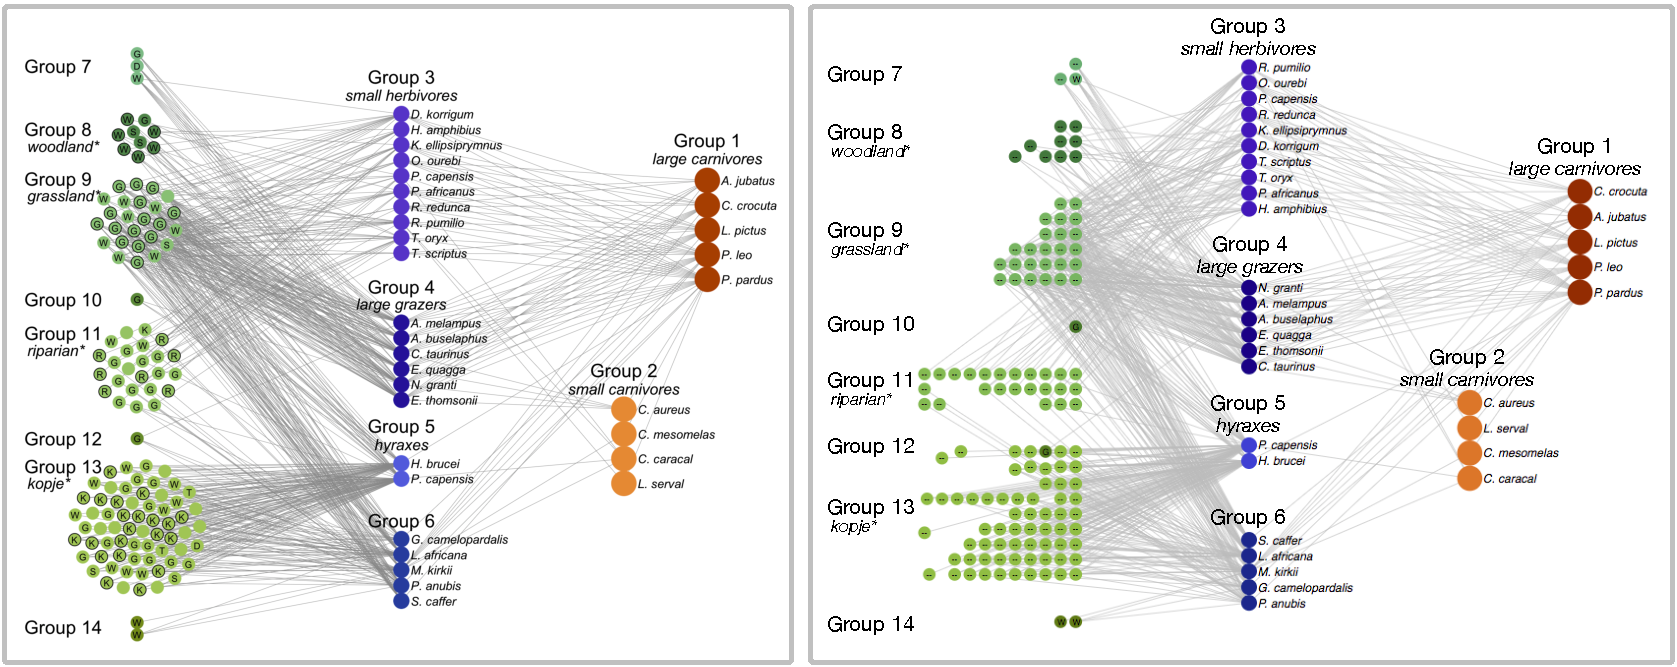
\includegraphics[width=\linewidth]{figures/serengeti-layout.pdf}
% 		\centering
% 	  \caption{\label{fig:teaser}}

% 	}
% }

\newcommand{\serengetiLayoutColumn}{
  \begin{figure}[t!]
    \centering
    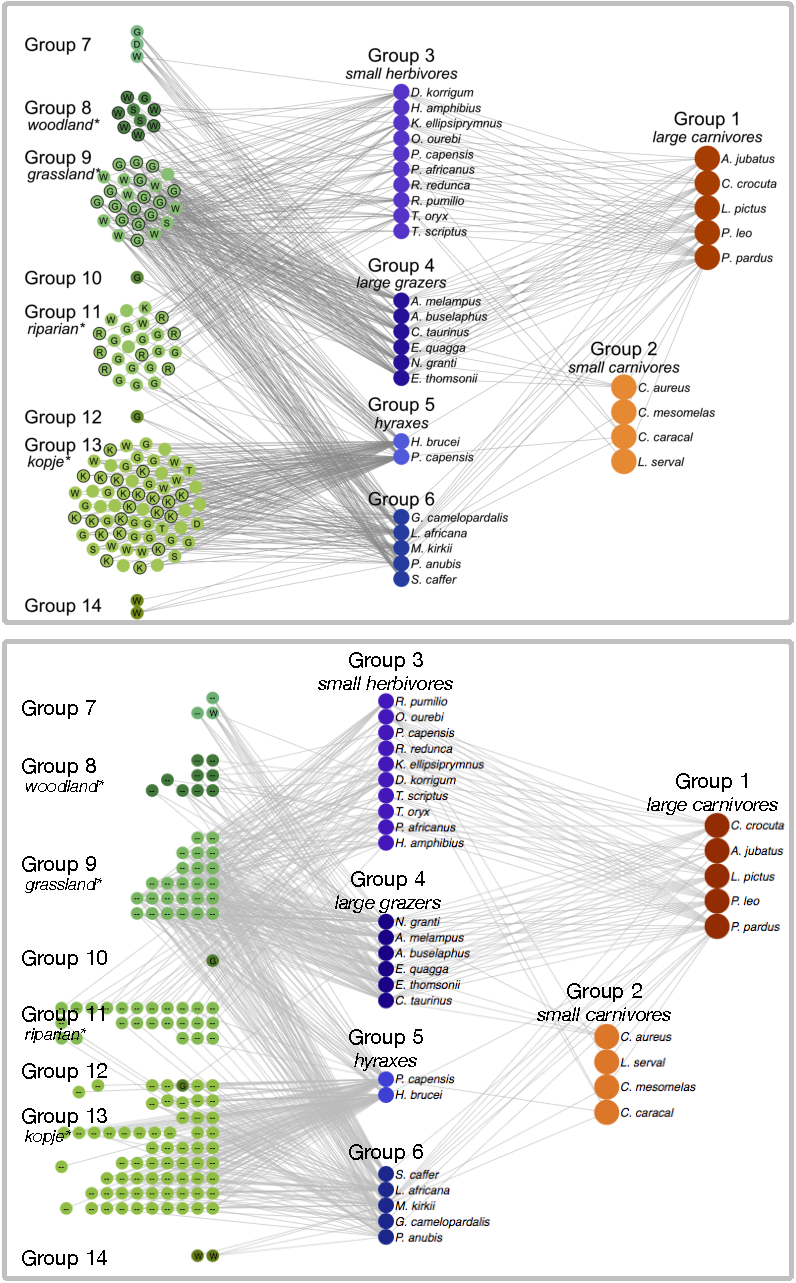
\includegraphics[width=0.81\columnwidth]{figures/serengeti-layout-column.pdf}
    {\caption{\label{fig:serengeti-layout}
    The layout for the Serengeti food web using our constraint language, as compared to Baskerville et al. \cite{baskerville2011spatial}.}}
    \vspace{-40px}
  \end{figure}
}

%%%%%%%%%%%%%%%%%%%%%%%%%%%%%%%%%%
%%%%%%%%%%%%% Design %%%%%%%%%%%%%
%%%%%%%%%%%%%%%%%%%%%%%%%%%%%%%%%%

\newcommand{\smallTreeExample}{
  \begin{figure}[t!]
    \centering
    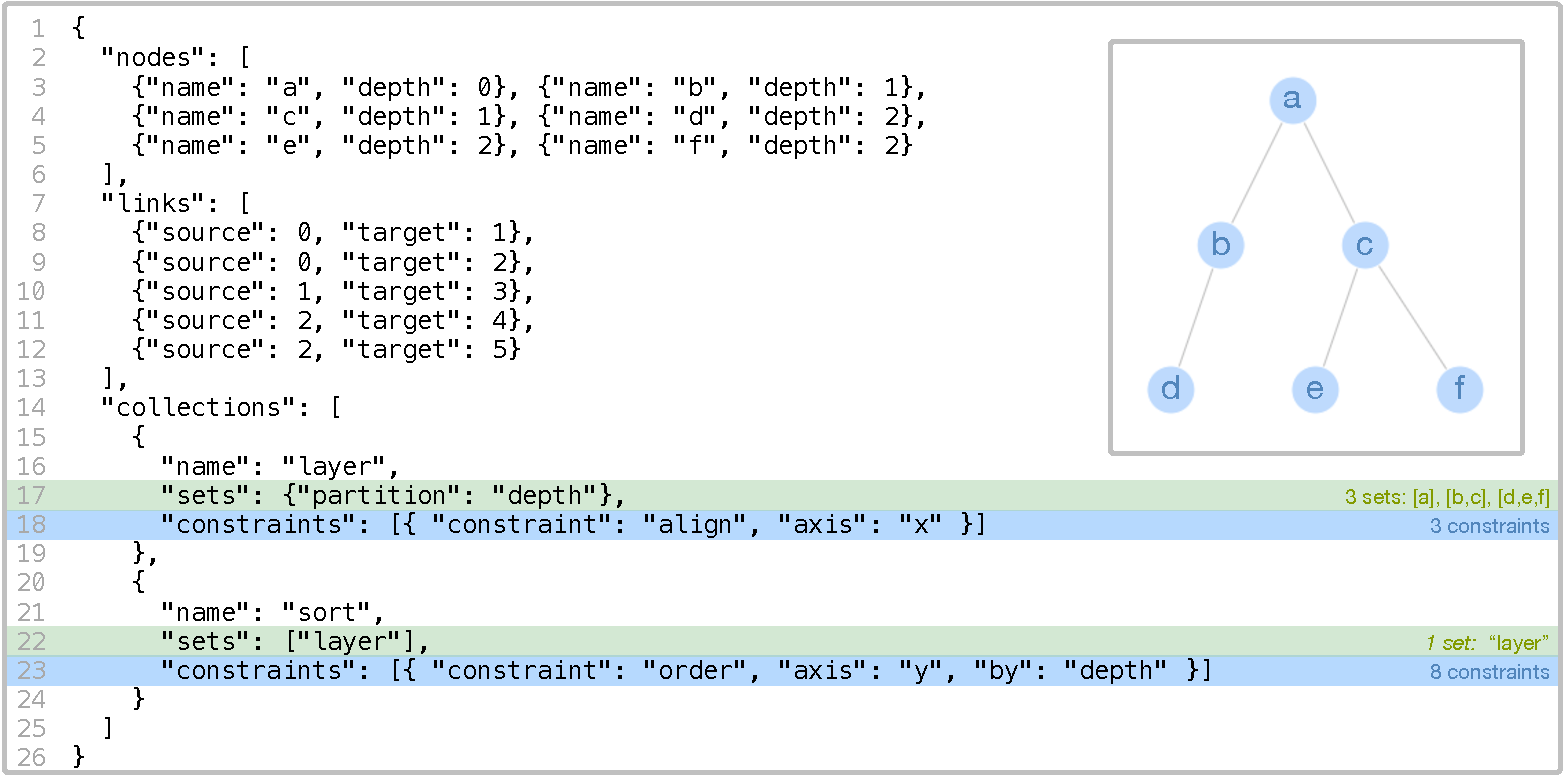
\includegraphics[width=\columnwidth]{figures/small-tree-example.pdf}
    {\caption{\label{fig:small-tree-example}
    The full \projectname\ specification for a small tree with six nodes. Nodes are split into sets based on their depth from the root \texttt{a}, and aligned. A new collection is formed containing the ``layer'' set and the layers are ordered by their depth to form the tree.
    }}
    \vspace{-20px}
  \end{figure}
}

\newcommand{\contradictionExample}{
  \begin{figure}[t!]
    \centering
    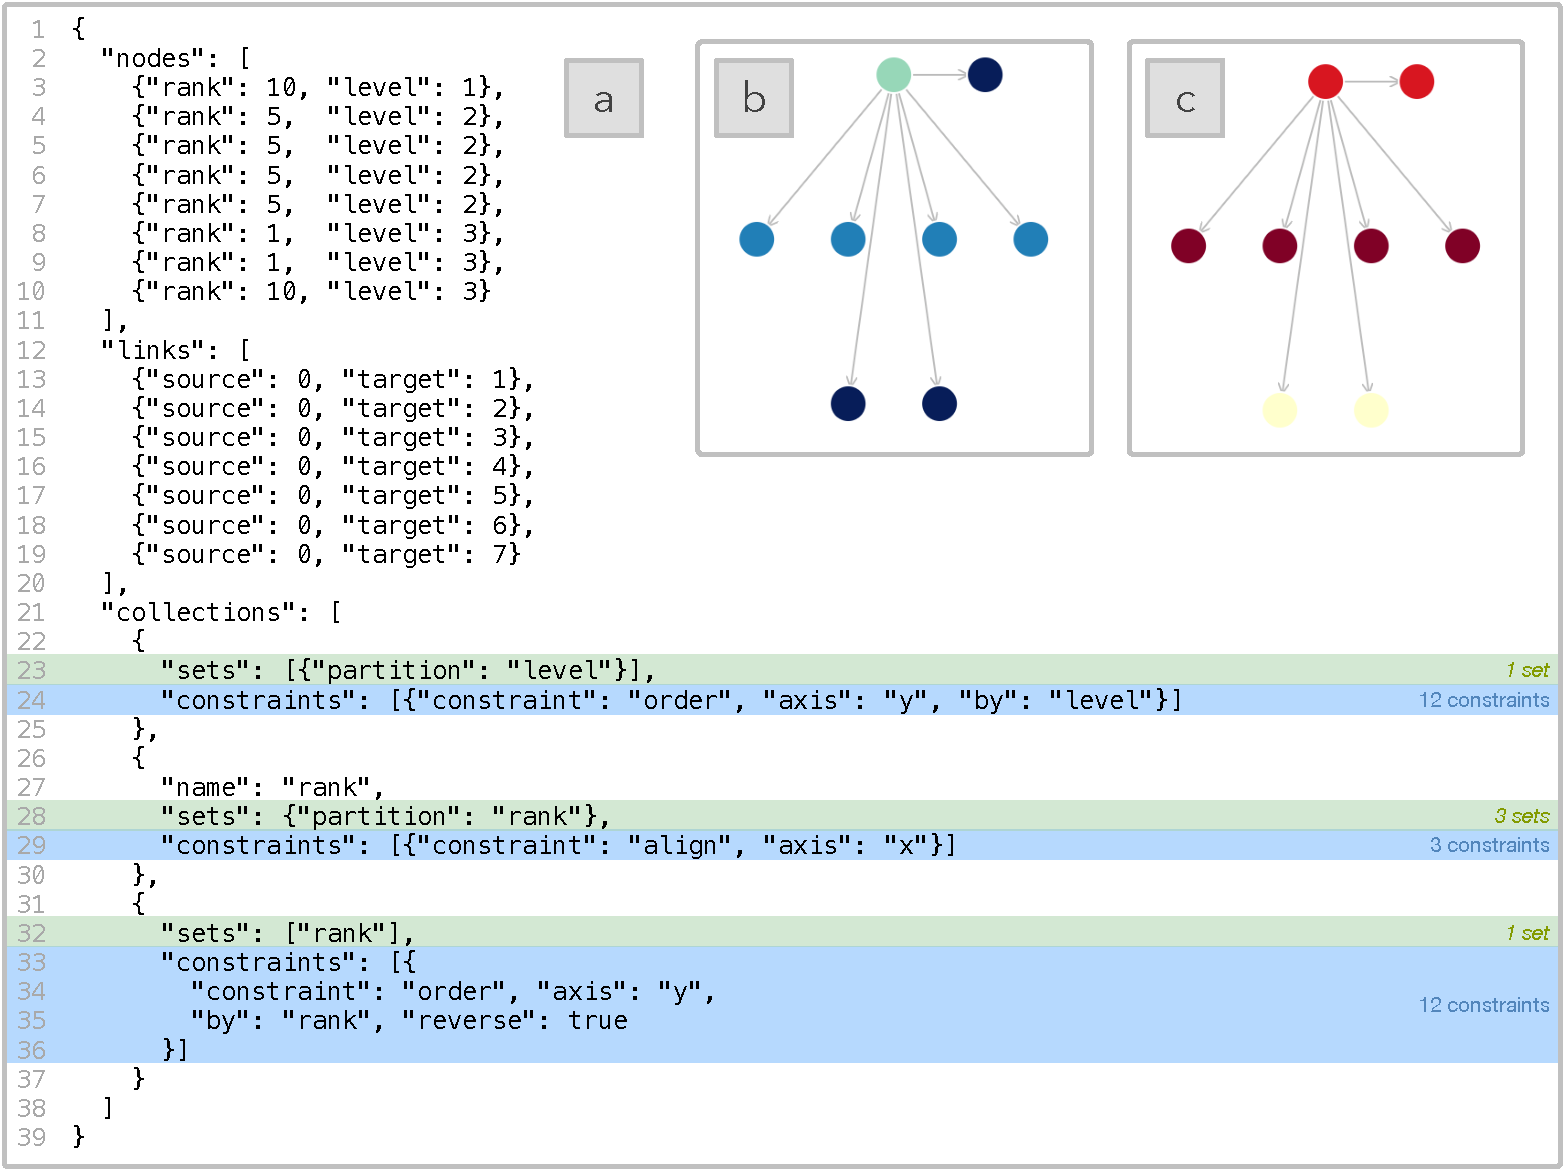
\includegraphics[width=\columnwidth]{figures/contradiction-example.pdf}
    {\caption{\label{fig:contradiction-example}
    (a) The full \projectname\ specification for a small graph with eight nodes. (b) Nodes are aligned based on their \texttt{rank}, and colored based on their \texttt{level}. Two constraints are applied to order the nodes, once by \texttt{level} and once by \texttt{rank}, which produces a contradiction. (c) Nodes are colored based on the amount of error for constraints that are invalid.
    }}
    \vspace{-20px}
  \end{figure}
}

%%%%%%%%%%%%%%%%%%%%%%%%%%%%%%%%%%
%%%%%%%%% Demonstration %%%%%%%%%%
%%%%%%%%%%%%%%%%%%%%%%%%%%%%%%%%%%

\newcommand{\krugerLayout}{
  \begin{figure}[t!]
    \centering
    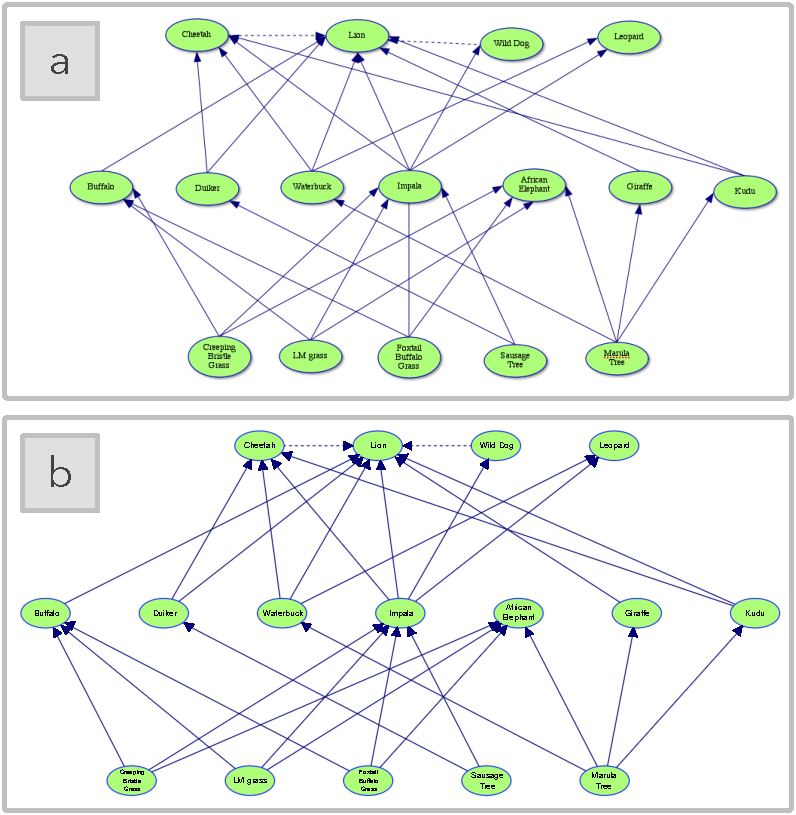
\includegraphics[width=0.81\columnwidth]{figures/kruger-layout.pdf}
    {\caption{\label{fig:kruger-layout}
    The layout for a small subset of the food web for Kruger National Park from (a) their website \orange{citation} as compared to (b) our layout using \projectname.}}
    \vspace{-20px}
  \end{figure}
}

\newcommand{\serengetiLayout}{
  \begin{figure*}[t]
    \centering
    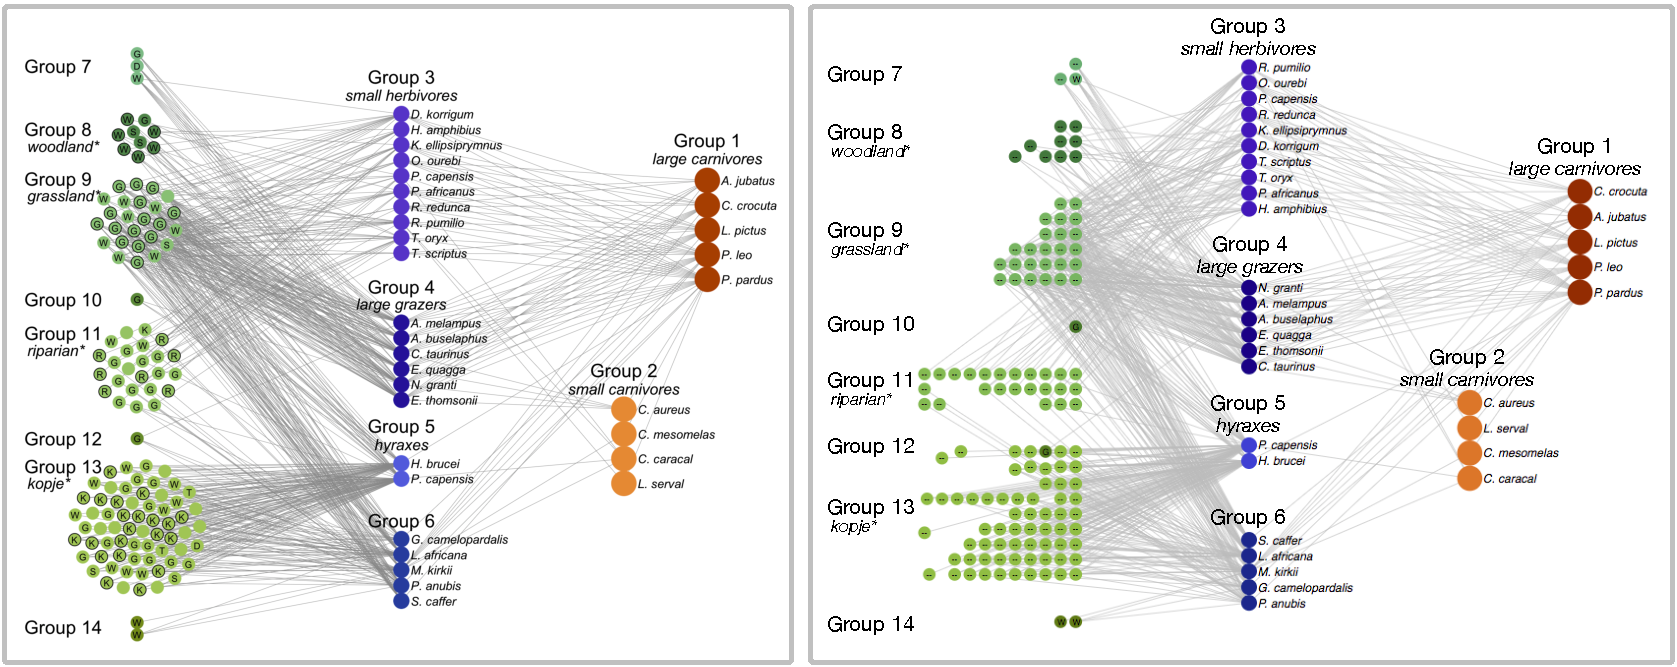
\includegraphics[width=\textwidth]{figures/serengeti-layout.pdf}
    \vspace{-20px}
    {\caption{\label{fig:serengeti-layout}
    The layout for the Serengeti food web using our constraint language, as compared to Baskerville et al. \cite{baskerville2011spatial}. \todo{retake photos on retina screen} \todo{label the two sides of the figure a/b}}}
  \end{figure*}
}

\newcommand{\serengetiSpec}{
  \begin{figure}[t]
    \centering
    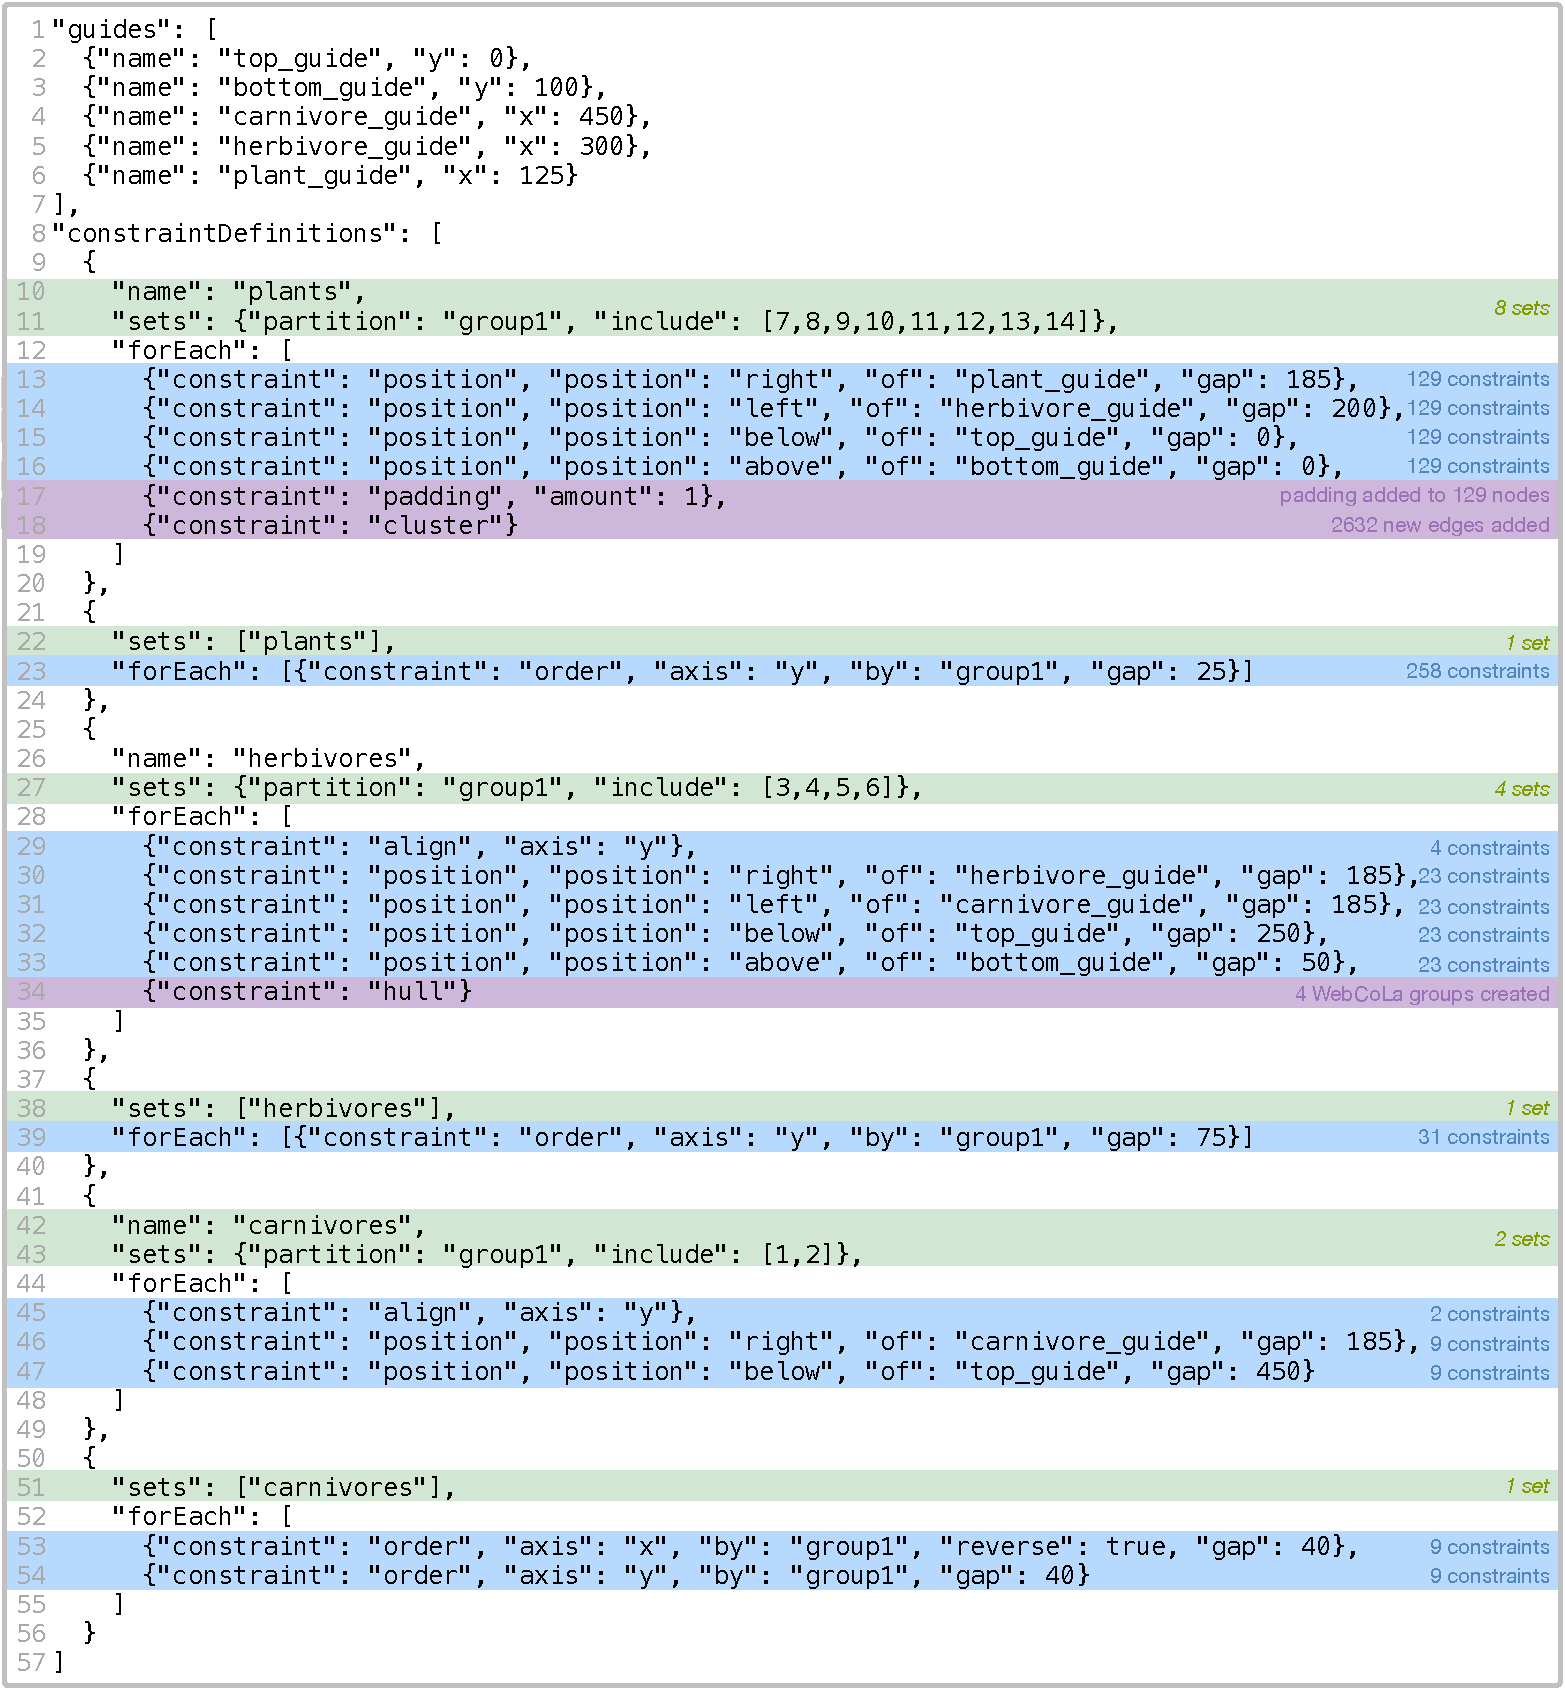
\includegraphics[width=\columnwidth]{figures/serengeti-spec.pdf}
    \vspace{-20px}
    {\caption{\label{fig:serengeti-spec}
    The \projectname~specification for the Serengeti food web shown in Figure~\ref{fig:serengeti-layout}. The code is annotated with the number of sets produced, the number of edges added, and the number of WebCoLa constraints generated for the final layout.}}
  \end{figure}
}

\newcommand{\syphilisLayout}{
  \begin{figure*}[t]
    \centering
    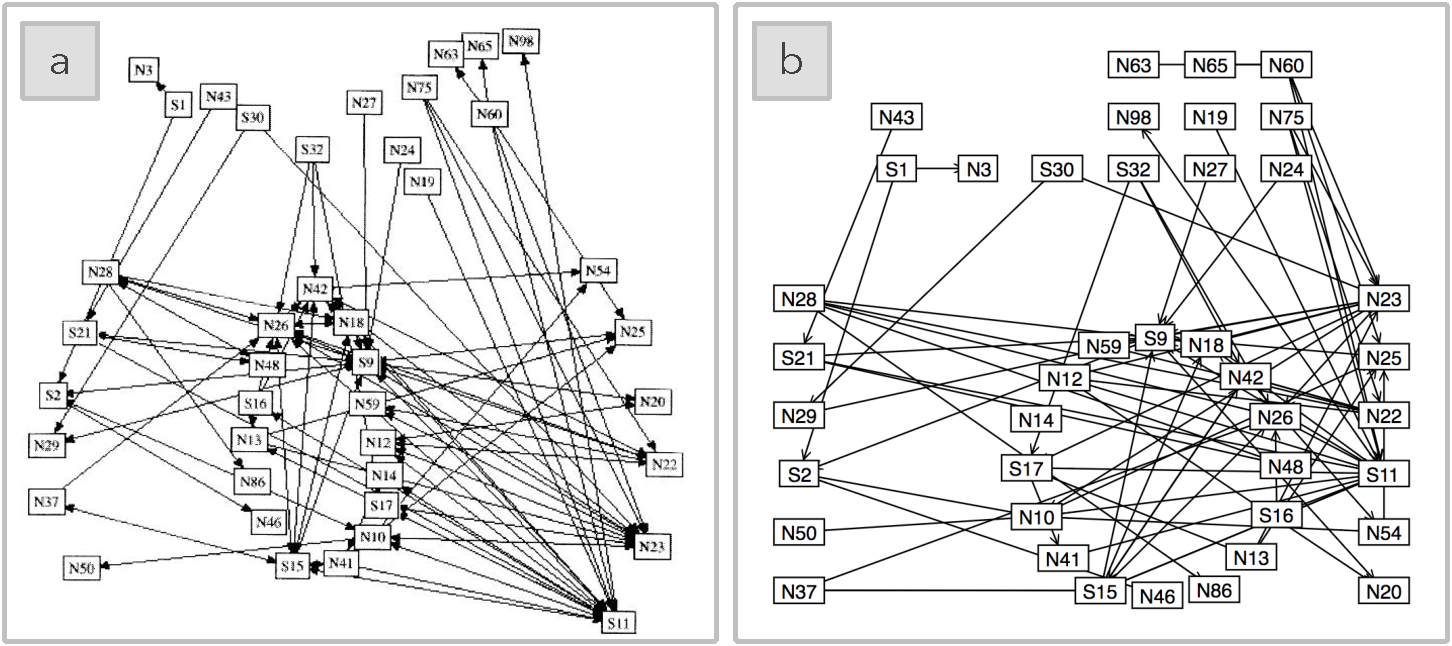
\includegraphics[width=\textwidth]{figures/syphilis-layout.pdf}
    \vspace{-20px}
    {\caption{\label{fig:syphilis-layout}
    The layout for the syphilis social network from (a) Rothenberg et al. \cite{rothenberg1998using} as compared to (b) the \projectname~layout. \todo{add some padding on the layout of the aligned men}}}
  \end{figure*}
}

\newcommand{\syphilisSpec}{
  \begin{figure}[t]
    \centering
    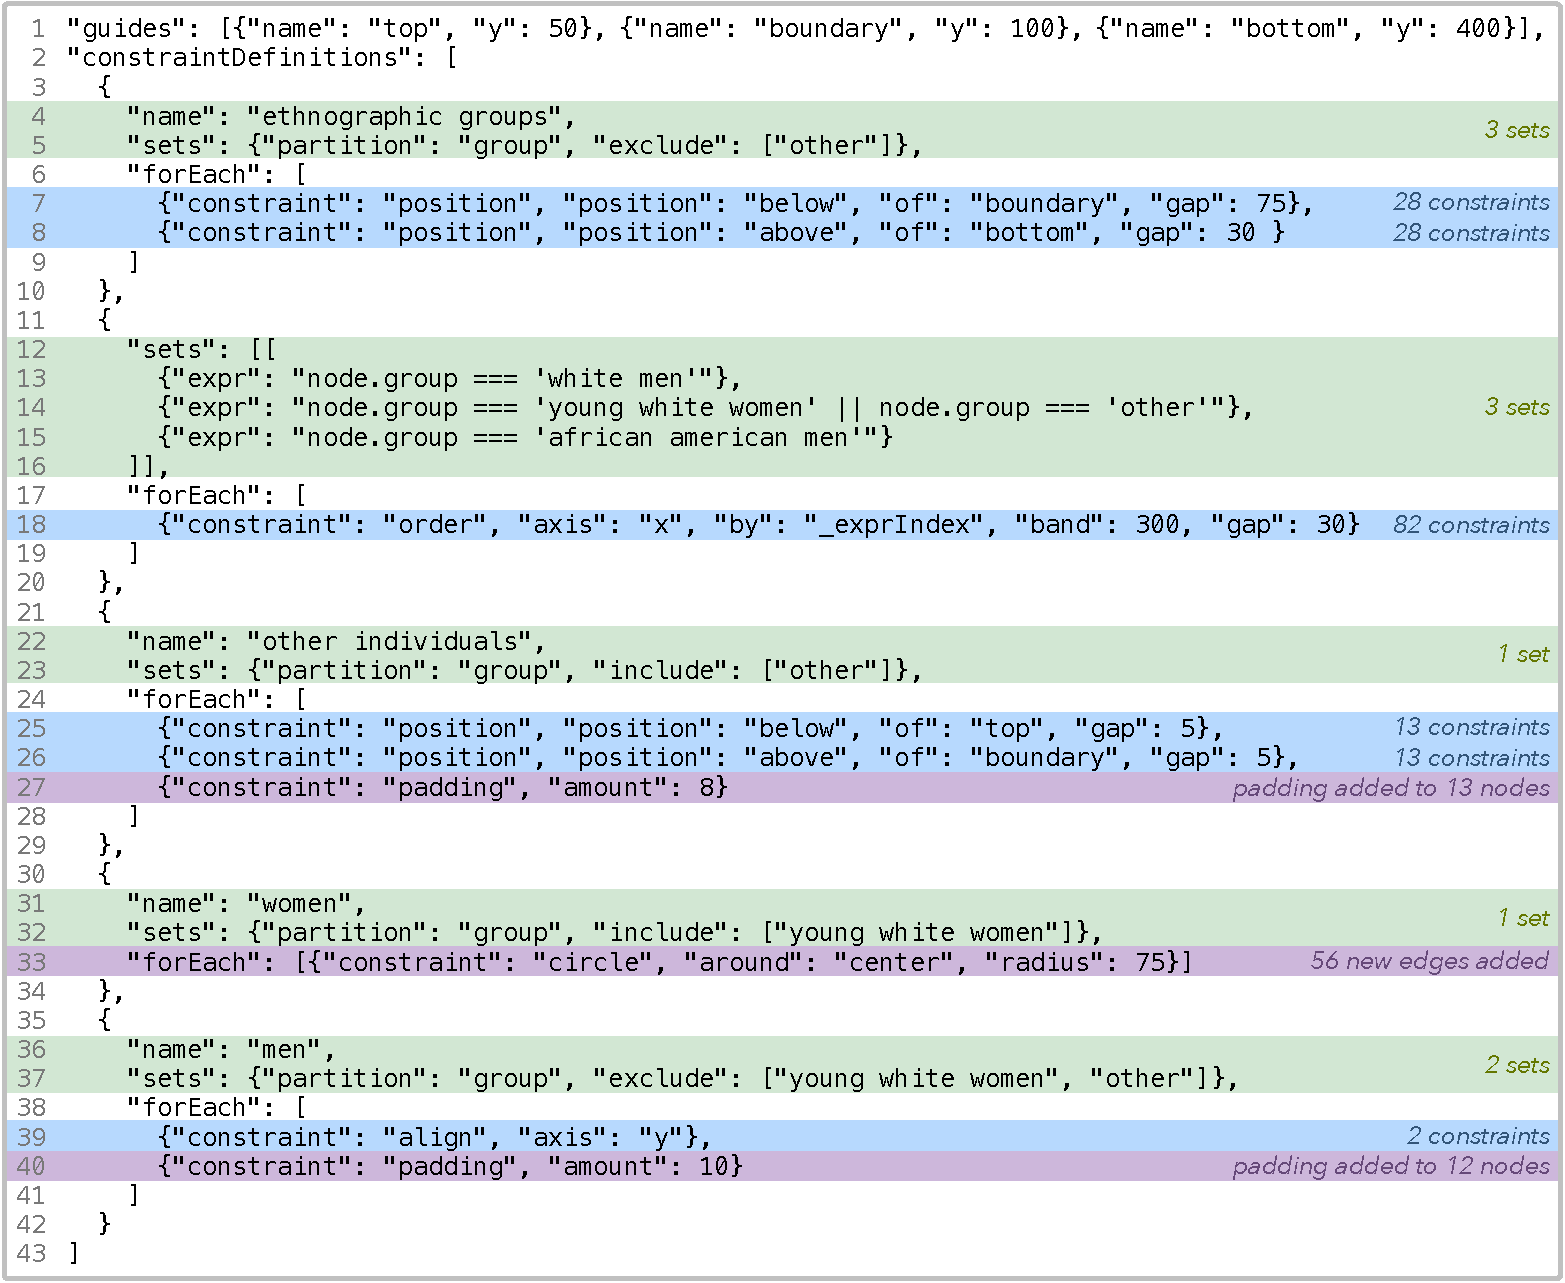
\includegraphics[width=\columnwidth]{figures/syphilis-spec.pdf}
    \vspace{-20px}
    {\caption{\label{fig:syphilis-spec}
    The \projectname~specification for the syphilis social network shown in Figure~\ref{fig:syphilis-layout}. The code is annotated with the number of sets produced, the number of edges added, and the number of WebCoLa constraints generated for the final layout.}}
  \end{figure}
}
\hyphenpenalty=100000

%-------------------------------------------------------------------------
\begin{document}

% \teaser{
%  \includegraphics[width=\linewidth]{eg_new}
%  \centering
%   \caption{New EG Logo}
% \label{fig:teaser}
% }

%\teaserFigure
\maketitle

%!TEX root = constraint-layout.tex
\newcommand{\paperabstract}{
Constraints enable flexible graph layout by combining the ease of
automatic layout with customizations for a particular domain.
However, constraint-based layout often requires many individual
constraints defined over specific nodes and node pairs.
In addition to the effort of writing and maintaining a large number
of similar constraints, such constraints are specific to the
particular graph and thus cannot generalize to other graphs in the same
domain. To facilitate the specification of customized and generalizable
constraint layouts, we contribute \projectname: a domain-specific language
for specifying high-level constraints relative to properties of the backing
data. Users identify node sets based on data or graph properties and apply
high-level constraints within each set. Applying constraints to
node sets rather than individual nodes reduces specification
effort and facilitates reapplication of customized layouts
across distinct graphs. We demonstrate the conciseness,
generalizability, and expressiveness of \projectname~on a series of
real-world examples from ecological networks, biological systems, and
social networks.
}

\begin{abstract}
  \paperabstract

  \begin{CCSXML}
	<ccs2012>
	<concept>
	<concept_id>10003120.10003145.10003146.10010892</concept_id>
	<concept_desc>Human-centered computing~Graph drawings</concept_desc>
	<concept_significance>500</concept_significance>
	</concept>
	</ccs2012>
	\end{CCSXML}
	\ccsdesc[300]{Human-centered computing~Graph drawings}
	\printccsdesc
\end{abstract}

%-------------------------------------------------------------------------
%!TEX root = constraint-layout.tex
\section{Introduction}
Graph visualizations can effectively represent properties of the underlying data structure, such as the hierarchy or connectedness of the data within the graph layout. Such visualizations are common across domains including ecological networks \cite{hinke2004visualizing,harper2006dynamic,lavigne1996cod,baskerville2011spatial,yodzis1998local,cohen2003ecological,kearney2016blog,benson2016higher}, biological systems \cite{barsky2008cerebral,shannon2003cytoscape,gehlenborg2010visualization,saraiya2005visualizing,becker2001graph}, and \orange{third example from demonstration}, among many others. In order to emphasize relevant trends in the data, the graph layout may utilize domain specific details; for example, in an ecological network, nodes could be split by trophic level (plant, herbivore, or carnivore) (Figure~\ref{fig:serengeti-layout}). This customized layout can more effectively reveal the feeding relationships between trophic levels and the hierarchical structure.

% Provide a bit more info about what the layout tools are doing - an additional setnece/rewording
% Not sure about 'layout tool' - cerebral is a midpoint between algorithm and customized
\todo{extend discussion of what the layout tools are doing (and tools might not be the right word/framing, algorithm seems better)}
Many domain specific layout tools have been developed to address particular graphing needs \cite{barsky2008cerebral,shannon2003cytoscape,kearney2017d3,kearney2017ecopath}. However, when a layout tool does not exist for the domain or task of interest, users are required to either fit their data to one of the available tools or create a customized layout of their own. Creating such a customized layout often requires both domain and programming expertise. \todo{unclear who is collaborating at this point.}
% Unclear who is collaborating at this point; a visualization expert?
When collaboration is infeasible, domain experts may be required to invest large amounts of time into learning the skills necessary to program the customized layout themselves. Furthermore, these customized tools are hard to generalize beyond their domain; these tools are carefully crafted to meet the needs of a particular domain or task, which means that it can be hard for domain experts to share their new programming expertise with others. This barrier to creating highly customized, domain specific layouts means there is a gap between the analysis needs of some domains and the availability of tools to handle those needs.

\todo{talk about constraint based solutions and the shortcomings before introducing our approach}

% See more about constraint based solutions and what are the shortcomings
% talk about tedium of cosntraint side - and the constraint based approaches

\todo{Need to come up with a careful, descriptive definition of what I mean by customized layouts at some point in the intro}
To enable the design of customized domain specific layouts with minimal programming expertise, we present a high-level constraint language for graph layout. Users partition nodes into sets based on node or graph properties and apply layout constraints within or between these sets. This approach allows users to specify layout requirements at a high-level, while deferring the computation of the node-level constraints to the underlying system. These constraint specifications reduce programming effort while still enabling highly customized and generalizable graph layouts. We demonstrate the utility of this technique with an implementation of our constraint language that compiles our high-level constraints into inter-node constraints for WebCoLa~\cite{WebCoLa}, a JavaScript library for constraint based graph layout. To demonstrate the ease and extensibility of our language, we recreate a number of customized layouts with our WebCoLa implementation. We show that users can compactly specify complex graph layouts that resemble those produced by customized layout engines.
%!TEX root = human-constraint-layout.tex
\section{Related Work}
There are many areas of related work surrounding the visualization and layout of graphs, and domain specific graphs in particular. Graphs are a common type of data seen across a variety of domains including social networks \cite{scott1988social,travers1967small,granovetter1973strength,watts1998collective,freeman1978centrality}, biological systems \cite{barsky2008cerebral,shannon2003cytoscape,gehlenborg2010visualization,saraiya2005visualizing}, and ecological networks \cite{hinke2004visualizing,harper2006dynamic,lavigne1996cod,baskerville2011spatial,yodzis1998local,cohen2003ecological,kearney2016blog,benson2016higher}. In this section, we identify some common tools for graph layout and describe some tools that have been tailored for domain specific tasks.

\subsection{Graph Visualization}
Graph layout has been a long-standing area of research and there are a number of common layout techniques for visualizing graph data including tree layouts or force-directed layouts. Graphviz \cite{ellson2001graphviz} and Gephi \cite{bastian2009gephi} are two examples of visualization engines specific to graph layout. D3.js \cite{bostock:d3} is a JavaScript library that provides a number of built in layouts for graph data including force-directed and hierarchical layouts. WebCoLa \cite{WebCoLa} is a JavaScript library for constraint-based layout that can be used alongside D3 or Cytoscape~\cite{shannon2003cytoscape}.

In addition to these standard layout techniques, there is a large field of related work surrounding graph layout techniques that emphasize particular aesthetic or structural properties in the graph. HOLA \cite{kieffer2016hola} presents a layout engine to produce layouts similar to those produced by hand by identifying common aesthetic properties of the graph used in manual layouts and using the results to drive the design of a new layout algorithm. Kieffer et al. \cite{kieffer2013incremental} present a constraint-based layout for creating graphs with node and edge alignment, and demonstrate the feasibility of such a technique in an interactive system, Dunnart \cite{dwyer2008dunnart}.

While these are some examples of customized layouts, the customization reflects general properties of the graph as opposed to domain specific details. Our work focuses on providing a general language for supporting customized graph layouts with minimal programming expertise.

\subsection{Domain Specific Graph Visualization}
\smallTree
To address the domain specific needs for graph analysis, a number of tools have been developed to utilize domain specific information in the layout. Cerebral \cite{barsky2008cerebral} is a tool designed to visualize biological systems and support interactive exploration of different experimental conditions. Cytoscape \cite{shannon2003cytoscape} is a visualization system designed to explore biomolecular interaction networks and provides a framework for accepting customized plugins to extend the system. Becker and Rojas \cite{becker2001graph} provide a customized algorithm for visualizing metabolic pathways. Kearney has developed D3 \cite{kearney2017d3} and Ecopath \cite{kearney2017ecopath} plugins to aid in the visualization of food webs.

Each of these tools was designed with a particular domain in mind to address the needs of domain experts who were unable to find the necessary support within existing tools. Our work aims to reduce the barrier of creating these customized systems by providing a compact way to specify domain specific graph layouts.

%!TEX root = constraint-layout.tex
\section{Design Considerations}

\todo{maybe it would be helpful to lay out the main design considerations
  for the language. e.g. talk about existing graph layouts and requirements
  when selecting or designing layouts by hand that could motivate our
  choice of constraints. Or would it be fine to just have this in the
  design section when discussing the rationale?}

%%%%%%%%%%%%%%%%%%%%%%%%%%%%%%%%%%%%%%%%%%%%%%%%%%%%%%%%%%%%%%
%%%%%%%%%%%%%%%%%%%%%%%%%%%%%%%%%%%%%%%%%%%%%%%%%%%%%%%%%%%%%%
\section{Design of \projectname}
\projectname\ is a domain-specific language for the creation of highly
customized graph layouts based on properties of the nodes. Users identify
element sets from the graph and apply constraints to all elements in a
given set. These sets can be hierarchically composed to create a flexible,
nested layout. \projectname\ reduces specification effort and allows the
user to focus on the graph layout in terms of high-level properties of the
data rather on individual nodes. These layout specifications can also be
easily reused across graphs for which the nodes have the same properties,
which allows the user to apply a single layout design across multiple
graphs in the same domain. In this section, we discuss the design of
\projectname\ including the process for specifying sets and applying
constraints.

\smallTreeExample

The main contribution of \projectname\ is the language for specifying
high-level constraints. \projectname\ specifications are composed of four
components: \emph{nodes}, \emph{links}, \emph{guides}, and
\emph{collections}. An example \projectname\ specification is shown in
Figure \ref{fig:small-tree-example}. Properties of the graph are included
as properties of the nodes and links. The user can then define collections
which are defined as a list of sets and a list of high-level constraints
that apply to the elements in each set of the collection. Users identify
\emph{sets} based on graph properties; sets can contain either graph nodes
or previously defined collections. Guides are an optional component and may
be used to define top-level layout boundaries (defined with an x and/or y
position), which can be referred to in the constraint specification.

%%%%%%%%%%%%%%%%%%%%%%%%%%%%%%%%%%%%%%%%%%%%%%%%%%%%%%%%%%%%%%
%%%%%%%%%%%%%%%%%%%%%%%%%%%%%%%%%%%%%%%%%%%%%%%%%%%%%%%%%%%%%%
\subsection{Specifying Sets in \projectname}
Each collection in \projectname\ is defined as a list of sets, where sets
are lists of elements. The elements in a set can be either nodes or
previously created sets, thus enabling a hierarchical composition of sets
for more complex layouts. In this language, we support several strategies
for specifying sets of nodes: \emph{partitioning}, \emph{expressions},
\orange{\emph{relations}}, and \emph{compositions}.

\textbf{Partitioning.} Users can partition all graph nodes into sets by
identify a property (\todo{Partition by multiple properties?}) of the nodes
with which to group the nodes (see Figure \ref{fig:small-tree-example},
Line \texttt{17}). Nodes are then separated into disjoint sets based on the
partition property. The user may also specify lists of values that identify
which property values to \texttt{include} or \texttt{ignore} when
performing the partition. These properties allow the user to create
partitions where some nodes are excluded from the partition, and are
therefore not placed in any of the partition sets.

\textbf{Expressions.} For more flexibility in the definition of sets, users
can specify a concrete lists of sets to compute using arbitrary boolean
expressions. For each expression, each node is evaluated based on the user
defined expression to determine if it is included in the set. The user may
refer to properties of the node using dot syntax (e.g.,
\texttt{node.<property>}). Users may also optionally specify a
\texttt{name} for the set, which may be used by the composition set
specification. For this specification strategy, it is possible to create
node sets that are not disjoint, and may thus produce unsatisfiable
constraints. \todo{example figure}

\textbf{Relations.} For some sets, it may be useful to identify particular
relationships between nodes, which can be specified as a relation. For each
node, \todo{finish this section}

\contradictionExample

\textbf{Compositions.} Sets may also be formed through the hierarchical
composition of collections. For example, in Figure
\ref{fig:small-tree-example} we first create a collection of sets using
partition on Line \texttt{17}, named ``layer.'' On Line \texttt{22} we
create a new collection that contains the ``layer'' set. Line \texttt{28}
and \texttt{32} of Figure \ref{fig:contradiction-example} show the same
strategy, whereas Line \texttt{23} shows the shorthand composition for
producing the collection containing one set. For compositions, the user may
refer to any named entities previously defined in the specification (e.g.,
collections or named sets produced from \emph{expressions}).

\todo{``from'' property for set specification?}

When a named set is defined, the set element promotes the properties that
are equivalent for all elements in the set to a property of the set
element. For example, in Figure \ref{fig:small-tree-example}, when the user
defines a partition on the nodes based on the \texttt{depth} (Line
\texttt{17}), then each set element is given a \texttt{depth} property with
the value for that set. This property may now be referred to in other parts
of the \projectname specification (e.g., Line \texttt{23}).


%%%%%%%%%%%%%%%%%%%%%%%%%%%%%%%%%%%%%%%%%%%%%%%%%%%%%%%%%%%%%%
%%%%%%%%%%%%%%%%%%%%%%%%%%%%%%%%%%%%%%%%%%%%%%%%%%%%%%%%%%%%%%
\subsection{Applying Constraints in \projectname}
\label{sec:constraints}
Once a collection has been defined, users can apply layout constraints to
each of the sets in the collection. We identify four different types of
constraints that can be applied to set elements: \texttt{alignment},
\texttt{position}, \texttt{order}, \texttt{circle}, and \texttt{unit}. In
the following sections, we describe the behavior and properties of each of
these constraints.

% design section: rationale for why these are the right constructs (sufficiently expressive)
	% why are they user friendly?
	% hypotheses and reason hope/belief/evidence

%%%%%%%%%%%%%%%%%%%%%%%%%%%%%%%%%%%%%%%%%%%%%%%%%%%%%%%%%%%%%%
\subsubsection{Alignment Constraints}
\constraint{\texttt{align} \emph{x} \texttt{axis}} Alignment constraints
specify the alignment of elements along an axis (Figure
\ref{fig:small-tree-example}, Line \texttt{18}). The constraint must
include the \texttt{axis} (e.g., \texttt{x} or \texttt{y}) on which the
elements should be aligned and may optionally include the
\texttt{orientation} for the alignment, one of: \texttt{center},
\texttt{left}, \texttt{right}, \texttt{top}, or \texttt{bottom}. When
applied to nodes, this constraint ensures that all the nodes are aligned
along the \texttt{axis}. When applied to sets, this constraint produces an
alignment based on the centroid or boundary of the set elements.

\emph{Rationale.} Alignment is a common characteristic seen when producing
graphs by hand \orange{citation} or utilizing particular layout strategies
\orange{citation} and is therefore crucial to support in \projectname.

%%%%%%%%%%%%%%%%%%%%%%%%%%%%%%%%%%%%%%%%%%%%%%%%%%%%%%%%%%%%%%
\subsubsection{Position Constraints}
\constraint{\texttt{position} \emph{right} \texttt{of}
  \emph{``top\_guide''}} Position constraints specify rules for the layout
of nodes relative to globally identified elements (\orange{figure}). The
constraint must identify a global element (e.g., a guide) to position the
set elements relative to and an orientation for the position (e.g.,
\texttt{left}, \texttt{right}, \texttt{above}, or \texttt{below}). The user
may optionally provide a \texttt{gap} for how far apart the elements should
be from the position element.

\emph{Rationale.} Position constraints allow the user to provide
overarching constraints relative to global elements such as guides. These
can be used to constrain the overall size of the graph or to section off
different areas. \todo{citations}

%%%%%%%%%%%%%%%%%%%%%%%%%%%%%%%%%%%%%%%%%%%%%%%%%%%%%%%%%%%%%%
\subsubsection{Order Constraints}
\constraint{\texttt{order} \emph{y} \texttt{axis} \texttt{by}
  \emph{``depth''}} Order constraints enforce a sort order on the set
elements (Figure \ref{fig:small-tree-example}, Line \texttt{23}). The
constraint must include the \texttt{axis} (e.g., \texttt{x} or \texttt{y})
on which the elements should be ordered. The constraint must also specify
the node property \texttt{by} which the order is determined. The user can
optionally define an explicit list of values for a custom
\texttt{order}. The user may also optionally include a boolean of whether
or not to \texttt{reverse} the order. Users may finally specify an optional
\texttt{band} property for the constraint that determines a size for each
set region; without the \texttt{band} property, the first and last elements
in the order are free to move on either end, whereas the \texttt{band}
enforces them to fit within the same sized space as the intermediate
elements.

\emph{Rationale.} Unlike position constraints, order constraints allow the
user to specify relationships between different sets of nodes to specify
the overall node layout. These relationships are particular useful for
sorting and hierarchical layouts on the different sets of nodes.

%%%%%%%%%%%%%%%%%%%%%%%%%%%%%%%%%%%%%%%%%%%%%%%%%%%%%%%%%%%%%%
\subsubsection{Circle Constraints}
\constraint{\texttt{circle} \texttt{around} \emph{``center''}} Circle
constraints allow the user to specify a ring layout for a set of
elements. The constraint must include which element the set elements should
be positioned around or may specify ``center'' for a generic center point
to be used.

\emph{Rationale.} Circular structures are a common layout requirement of
existing strategies \orange{citation} and can be crucial for relating
properties of the underlying structure.

%%%%%%%%%%%%%%%%%%%%%%%%%%%%%%%%%%%%%%%%%%%%%%%%%%%%%%%%%%%%%%
\subsubsection{Unit Constraints}
\constraint{\texttt{unit}} Unit constraints specify additional layout
properties for elements in the set. The user may optionally specify a
boolean \texttt{enclose} that prevents the set elements from overlapping
with other sets (\orange{figure}). The user may optionally specify an
\texttt{attract} property as either \texttt{center}, \texttt{left},
\texttt{right}, \texttt{top}, or \texttt{bottom} that causes the nodes to
be drawn to the specified area of the set (\orange{figure}). An optional
\texttt{padding} property determines the minimum amount of spacing that
should exist between elements in the unit and finally an optional
\texttt{spacing} property determines whether the spacing is either
\texttt{free} or \texttt{fixed}.

\emph{Rationale.} The unit constraint allows the user to enforce more
control on how the nodes within a set behave outside of the general layout
constraints specified earlier. These constraints allow the user to apply
more nuanced behaviors between the nodes.

%%%%%%%%%%%%%%%%%%%%%%%%%%%%%%%%%%%%%%%%%%%%%%%%%%%%%%%%%%%%%%
\subsection{Unsatisfiable Constraints in \projectname}
For a \projectname\ specification, it is possible to create node sets that
are \emph{not} disjoint and may thus be easily susceptible to the
specification of unsatisfiable constraints. Furthermore, through various
combinations of set specifications and constraint applications, it is
possible for the user to specify unsatisfiable constraints in the
\projectname\ layout. An example of a layout with unsatisfiable constraints
is shown in Figure \ref{fig:contradiction-example}. This layout completes
two partitions of the nodes (once by \texttt{level} and once by
\texttt{rank}); these collections lifted and an order constraint is applied
to enforce a hierarchy between the sets. However, due to the properties of
the nodes, the node with \texttt{rank 10} and \texttt{level 3} faces a
contradiction in the layout. Figure \ref{fig:contradiction-example}c shows
the error on the nodes that have constraints unsatisfied by the layout
(where darker means more error).

\todo{Does it make sense to talk about this here, or should we provide this
  as an example that we talk about later? Or should we talk about it more
  generally without an example and discuss why this is
  allowed?}\\ \\ \\ \\ \\ \\ \\ % Line breaks because latex is mad for some reason

%!TEX root = human-constraint-layout.tex
\section{High-Level, User-Defined Constraints}
\smallTree
In this section we describe our constraint language for high-level, user-defined constraints. This languages includes support for specifying sets of nodes over which to run the constraints and three types of constraints over the nodes: \emph{alignment}, \emph{order}, and \emph{position}. Figure \ref{fig:small-tree} shows a small example specification for a tree layout and the resulting six node tree. 

We refer to two types of constraints throughout this paper: \emph{high-level} constraints and \emph{layout} constrains. \emph{High-level} constraints identify sets over which node-specific \emph{layout} constraints are applied. Every \emph{high-level} constraint must include a \texttt{"name"} property and specify sets over which to apply the \emph{layout} constraints. However, \emph{layout} constraints for a \emph{high-level} constraint are optional; in cases where \emph{layout} constraints are not provided, the user may simply want to define sets of nodes to refer to later in her constraint specification.

\subsection{Specifying Sets}
\label{sec:sets}
Every high-level constraint must specify a group of sets over which the layout constraints are defined. There are two types of high-level constraints that can be specified: \emph{within set} constraints and \emph{between set} constraints. \emph{Within set} constraints describe constraints that are applied to all of the nodes within a given set whereas \emph{between set} constraints describe constraints that are between larger sets. We describe how to define each type of constraint and show examples of how these constraints are applied.

\subsubsection{Within Set Constraints}
The user specifies within set constraints with the \texttt{"set"} property as shown for \texttt{alignLayer} in Figure \ref{fig:small-tree}. There are two ways to specify sets for within set constraints: the user can either partition all the nodes into disjoint sets or the user can specify expressions to create specific sets of nodes.

The simplest set definition is to \texttt{"partition"} nodes into sets based on a property of the node. When generating the sets, the system extracts the property of the node to use as the key for the set. Using \texttt{"partition"}, nodes can only occur in one set specification for the given constraint.

There are two additional properties that users can apply to set partitioning: \texttt{"include"} and \texttt{"ignore"}. \texttt{"include"} allows the user to specify a property of the accepted node to \emph{include} in the set. This property must also be a node, for example the \texttt{"parent"} or \texttt{"firstchild"} of the node \green{add a figure that shows this}. \texttt{"ignore"} represents a list of keys to \emph{ignore} when creating the sets. This property can be useful for preventing nodes with specific properties from being included in the layout (e.g. the \texttt{layer} constraint of Figure \ref{fig:tlr4-layout}).

Alternatively, the user can specify a concrete list of sets to compute. In this representation, the user defines an expression that returns a boolean value of whether or not the node should be included in the set. The user may also specify an optional \texttt{"name"} property that is used by the debugging tools. Using this syntax, users may specify sets such that a node can appear in multiple sets. However, we currently throw an error when such a specification occurs. Future work is required to determine whether or not this behavior would be useful for complex layouts. The \texttt{"expr"} definition currently supports value comparisons (e.g. \texttt{==}, \texttt{<=}, \texttt{>}), and conjunctions (\texttt{\&\&}) and disjunctions(\texttt{||}) of value comparisons and boolean values. The user may use \texttt{datum.property} to refer to properties of the node.

Within set constraints define constraints that should be applied to all nodes in a set separate from nodes outside the set. In Figure~\ref{fig:small-tree}, the user partitions nodes into sets based on their depth and creates an \emph{alignment} constraint to align the nodes in each set along the x-axis.

\subsubsection{Between Set Constraints}
The user specifies between set constraints using the \texttt{"from"} property as shown by the \texttt{orderLayers} constraint in Figure~\ref{fig:small-tree}. The user specifies between set constraints as a list of previously named constraints. Between set constraints define constraints that should be applied between sets but not between nodes in a given set. In Figure~\ref{fig:small-tree}, the user selects all the sets defined by \texttt{alignLayer} and creates an \emph{order} constraint to sort the sets by their depth along the y-axis.

\subsection{Specifying Constraints}
Once the user has defined sets of nodes over which to apply the constraints, she may optionally define layout constraints for that specification. Every cosntraint must have a \texttt{"type"} property that defines the type of constraint. We support three types of layout constraints: \emph{alignment} (\texttt{"align"}), \emph{order} (\texttt{"order"}), and \emph{position} (\texttt{"position"}).

\subsubsection{Alignment Constraints}
Alignment constraints are the easiest constraint to specify in our constraint language and define using WebCoLa. Alignment constraints must have two properties, \texttt{"type"} and \texttt{"axis"}. The property \texttt{"axis"} can be defined as either \texttt{"x"} or \texttt{"y"}. Figure~\ref{fig:small-tree} shows an example of \emph{alignment} for the high-level constraint \texttt{alignLayer}.

\subsubsection{Order Constraints}
Order constraints have three required properties: \texttt{"type"}, \texttt{"axis"} (either \texttt{"x"} or \texttt{"y"}), and \texttt{"by"}. The property \texttt{"by"} defines the property with which to order the nodes. If the \texttt{"by"} property does not have an obvious ordering (e.g. numeric, alphabetical), the user may optionally define an \texttt{"order"} property that is an ordered list of the expected inputs to the ordering function. The user may also optionally define a \texttt{"reverse"} property to reverse the behavior of the ordering. Figure~\ref{fig:small-tree} shows an example of an \emph{order} constraint for the high-level constraint \texttt{orderLayers}, which forces the layers to be positioned along the y-axis based on their depth.

\subsubsection{Position Constraints}
Position constraints have three required properties: \texttt{"type"}, \texttt{"position"}, and \texttt{"of"}. The property \texttt{"position"} accepts the values \texttt{"right"}, \texttt{"left"}, \texttt{"above"}, or \texttt{"below"}. The \texttt{"of"} property can be defined as a node, for example the \texttt{"parent"} or \texttt{"firstchild"} of the current node, or as a temporary point. The temporary point definition can include any combination of the properties \texttt{"name"}, \texttt{"x"}, and \texttt{"y"}. If \texttt{"x"} or \texttt{"y"} is not defined, it is initialized to zero by default. Specifying a \texttt{"name"} property allows the new node to be reused in different parts of the specification. The temporary nodes are optionally visualized in the layout and can be used to modify the final layout by moving the nodes. An example of this behavior is shown in Figure \ref{fig:serengeti-iterations}b,c.

\subsection{Built-in Properties}
The constraint specification can use any properties of the nodes in the original graph. However, we also provide a number of built-in properties that can be defined over the nodes. These properties are automatically computed and added to the graph specification prior to computing the final WebCoLa constraints. These properties are only added to nodes if such a property does not already exist on the nodes.

\begin{description}
\item[\texttt{\_id}] The index of the node in the graph specification.
\item[\texttt{depth}] One more than the max depth of the node's parents. This property is only allowed if the graph contains only one root node and does not contain cycles.
\item[\texttt{parent}] The parent of the current node. This property is only allowed if the node has one parent or is defined as the parent with the smallest \texttt{"\_id"}.
\item[\texttt{firstchild}] The child node of the current node with the smallest \texttt{"\_id"}.
\item[\texttt{parents}] The list of nodes that have edges where the current node is the target.
\item[\texttt{children}] The list of nodes that have edges where the current node is the source.
\item[\texttt{neighbors}] The list of nodes that have edges connected to the current node. This property is the join of the \texttt{"parents"} and \texttt{"children"} properties.
\item[\texttt{degree}] The number of \texttt{"neighbors"}.
\end{description}

%!TEX root = constraint-layout.tex
\section{Examples Reproduced in \projectname}
\label{sec:examples}

To demonstrate the simplicity and generalizability of \projectname, we
reproduce several real-world examples from ecological
networks~\cite{baskerville2011spatial}, biological
systems~\cite{barsky2008cerebral}, and social
networks~\cite{rothenberg1998using}. We compare our recreated
visualizations to the origianl layouts and discuss the benefits of our
technique for creating highly customized graph layouts.

\todo{Do we want to include disclaimers somewhere in this section that not
  all the recreations may be an exact match to those seen due to
  transcription errors or lack of information available in the original
  publication?}

\todo{At least one of the demonstrations we include should show that we can
  reuse a graph specification across graphs with similar properties.}

% running example in design section?

% comparison of user spec and generated spec (quantiative comparison)
% point out measure of comprehension
% our demo uses domain props whereas low-level constraints in _id (separate from original intent)

% simplicity and generalizability --> conciseness and expressiveness
%     (efficiency or learnability are other ideas)
% 2b spacing on nodes
% syphilis (does circle order matter?)


\subsection{Serengeti Food Web}
\krugerLayout
\serengetiLayout
\serengetiSpec

Food webs visualize complex producer-consumer relationships in ecological
systems and are a common presentation strategy for this information
\cite{hinke2004visualizing,harper2006dynamic,lavigne1996cod,baskerville2011spatial,yodzis1998local,cohen2003ecological,benson2016higher,kruger2017}
\orange{kruger citation} despite the challenge of creating an informative
visualization \cite{kearney2016blog}. Small or simplified food webs may be
drawn by hand, but many real world ecosystems can have hunderds of
interconnected organisms. In such cases, a customized layout may be useful
for reasoning about the structure of the ecological system.

Small food webs exhibit several of the properties of larger food webs, such
as a hierarchy arranged by the trophic level of the individuals in the
network. For example, the figure for Kruger National Park includes a simple visualization
of such relationships for a subset of the species found in the park
(Figure~\ref{fig:kruger-layout}a). We can easily recreate the layout with a
small number of constraints on the nodes (Figure~\ref{fig:kruger-layout}b);
in particular, we constrain each trophic level to be aligned and enforce an
ordering of the layers that respects the food web hierarchy. This
\projectname specification could easily be applied to other food webs to
produce a similar layout. \todo{this could be an easy place to have a
  second small food web with the same spec/layout?}. However, as the food
web gets more complex, it becomes necessary to relax the alignment
constraints or introduce additional clustering to highlight other
structures within the layout.

One example of a larger ecological network is the Serengeti food web from
Baskerville et al.~\cite{baskerville2011spatial}, which depicts the
relationships among 161 plants, herbivores, and carnivores with 592 links
between entities. Baskerville et al.\ use a Bayesian analysis method to
identify group structure for the Serengeti food web, and provide a
customized layout of their results showing both the trophic hierarchy and
the clustering of the groups (Figure \ref{fig:serengeti-layout}a). This
analysis approach and visualization highlight relationships between plant
habitats and the underlying network structure that may be hard to identify
from the data alone.

We recreated the Serengeti food web visualization in
\projectname~(Figure~\ref{fig:serengeti-layout}b), using the specification
shown in Figure \ref{fig:serengeti-spec}. \todo{include a description of
  what the specification is doing, what constraints we use, and the
  statistics for the final layout.} \todo{Maybe include something like
  Fig. 7 from the class paper?}

The original visualization was published in \textsc{Plos} Computational
Biology \cite{baskerville2011spatial}, and an interactive version of the
figure was created with D3 \cite{baskerville2011interactive}. The
interactive version of the figure lacks the labeling and alignment of the
published figure, but allows the viewer to more easily trace the links
between different nodes in the network. With \projectname, the layout
structure is specified by the constraints, which could support similar
interactive behaviors while maintaining the structural features of the
published figure.

Baskerville et al.\ note that \emph{``We have not included invertebrates
  (insects and parasitic helminths) or birds''} in their published food
web, though \emph{``hypothesize that the general conclusions will be
  largely robust to the addition of more species.''} One advantage of
\projectname~is that the layout is independant of the individual nodes, so
the authors could easily reuse this layout to visualize future iterations
of the Serengeti food web or to explore similar structures across different
ecological communities.

\subsection{TLR4 Network}
\tlrfourSpec

\todo{Write section about tlr4 network}

\subsection{Syphilis Social Network}
\syphilisLayout
\syphilisSpec

\todo{Jeff noted that the nodes in the circle do not have the same order -
  did they have an important order before worth capturing, if so, what?}

Social networks can be a powerful way to understand inter-personal
relationships and are useful for tracking the spread of diseases that
result from personal contact \cite{rothenberg1998using} \orange{[other
    citations]}. The ability to track and identify individuals at risk can
help lead to treatment and help manage the spread of the disease. In
addition to the links between individuals, structuring the graph layout by
properties such as ethnic group may reveal additional details about the
spread of the disease.

Rothenberg et al.\ discuss an ethnographic approach to identifying the
``core'' groups in a social network to better understand the transmission
of syphilis amongst sexual partners~\cite{rothenberg1998using}. They found
that there were three primary groups involved -- affluent white men (ages
17-21), young white women (ages ??-??), and African-American men (ages
16-??), which are visualized from left to right in Figure
\ref{fig:syphilis-layout}a. The authors note that a number of outsiders
(visualized as the top cluster of Figure \ref{fig:syphilis-layout}a) to
these ``core'' groups played a significant role in the network. In
particular, \emph{``Visualization of these groups and all their sex
  partners uncovered the importance of several people not specifically
  identified with these groups (e.g., N43 and S30) who served as bridges
  between the two groups of men.''}

\todo{I don't have the N43 bridge link in my visualization as that was not
  clear from any of the figures in their paper...}

We reproduced this example with
\projectname~(Figure~\ref{fig:syphilis-layout}b) and included a number of
additional constraints on the layout (Figure~\ref{fig:syphilis-spec}) apart
from the separation constraints that are visible in the original image. In
particular, we included a circle constraint on the group of young white
women to more strongly enforce the result shown in the original figure and
applied an alignment constraint on the two groups of young
men. \todo{discussion of the statistics for the final layout.}

\subsection{\orange{<<Fourth example>>}}
\todo{Another example with more reusability / different layouts}

%!TEX root = human-constraint-layout.tex
\section{Discussion and Future Work}
In the previous section we showed a few example use cases of our constraint language for various types of graph layout. In this section we talk about some of the lessons learned from this process, our current implementation strategies, and areas for future work on this project.

\subsection{Adding Customized Annotations}
Creating a domain specific layout generally requires both a domain expert and individual with programming expertise. The domain expert provides knowledge about the desired layout motivated by the underlying graph properties whereas the programmer provides the expertise to actually compute the desired layout algorithm. In some cases, the domain expert may also strive to act as the programmer, but taking on such a role may require large amounts of time and effort on behalf of the domain expert.

The goal of this work is to provide a compact language in which to specify domain specific layouts. In the previous section, we showed that we can feasibly recreate complex domain specific layouts with a compact layout specification. However, as is evident from the comparisons (Figure \ref{fig:serengeti-layout}, \ref{fig:tlr4-layout}), the user may want to incorporate additional information via node labeling, group labeling, or other annotations on the visualization. Our system does not currently provide support for such customizations. Future work may want to examine how to incorporate layout driven annotations.

\subsection{Constraint Specification Syntax}
In future iterations of this constraint language, we need to revisit some areas of the current constraint syntax to ensure that constraints are both understandable and expressive. There are two aspects of the current syntax that require additional work: specifying constraints and specifying sets.

\subsubsection{Specifying Constraints}
We identified two styles of high-level constraints, \emph{within set} constraints and \emph{between set} constraints, which represent different techniques for applying constraints over sets of nodes (see Section \ref{sec:sets}). In an earlier iteration of our constraint language, we defined a high-level constraint as follows:

\begin{verbatim}
        {
          "name": NAME,
          "set": SET,
          "within": [CONSTRAINTS...],
          "between": [CONSTRAINTS...]
        }
\end{verbatim}

In our final constraint language, we decided to standardize the specification of layout constraints using the \texttt{"constraint"} syntax rather than \texttt{"within"} and \texttt{"between"} in order to support more customizable constraint specifications, instead varying the type of constraints via the \texttt{"set"} or \texttt{"from"} definition for the high-level constraint. However, in all of the examples shown in this paper, there is a tight relationship between the sets used for \emph{within set} and \emph{between set} constraints (Figure \ref{fig:small-tree}, \ref{fig:tree-layout}, \ref{fig:serengeti-layout}, \ref{fig:small-foodweb-layout}, \ref{fig:tlr4-layout}). Future work is required to understand if standardization is appropriate or if a syntax like the one shown here would be more understandable.

\subsubsection{Specifying Sets}
Future work is also required to explore how best to specify sets in our language. We described a number of techniques for specifying sets including \emph{partitioning} and \emph{manual specification} via predicates (see Section \ref{sec:sets}).

For the \emph{partitioning} approach the user can include additional properties \texttt{"include"} and \texttt{"ignore"} to modify which nodes are selected for a given set and which sets are excluded from the partitioning; however, while these properties sound similar from a linguistic standpoint, it is important to note that they do not operate on the same aspects of the graph and thus do not have reflexive behaviors. Each of these properties was initially introduced to target particular use cases for graph layout, but in future iterations it may be useful to revisit the set specification to create a more straightforward and understandable syntax.

The process of \emph{manual specification} for sets using the \texttt{"expr"} syntax also introduces a potential problem in that the sets do not enforce a disjoint partition of the nodes; in other words, it is currently possible to specify sets using this syntax that include overlapping nodes. This limitation means that it is possible for users to specify constraints that are impossible to satisfy. Additional research is required to determine if there are benefits from supporting overlapping sets or if the manual specification syntax should warn against or disallow such specifications from occurring.

\subsection{Generating Constraints and Optimizations}
The current process of generating WebCoLa constraints from our high-level constraints is unoptimized (see Table \ref{tab:numConstraints}). There are a few optimizations that can be made in particular that can help to reduce the number of WebCoLa constraints.

\emph{Between set alignment} constraints currently force all the nodes across all the sets to become aligned. An improvement would be to use an iterative layout that produces the inter-set layout before positioning the set as a whole. This strategy would significantly reduce the number of constraints that need to be solved by the underlying system and produce a more expected layout for the specified constraint.

\emph{Order} constraints currently produce constraints between pairs of nodes, ignorant of the desired ordering. One optimization is to reflect the ordering in the constraint generation process to only produce constraints for neighboring nodes. For \emph{within set} constraints, this strategy would only apply constraints between adjacent nodes in the final order. For \emph{between set} constraints, we could include an optimization to use temporary nodes to enforce the order rather than combinatorially producing constraints between pairs of nodes.

\emph{Between set position} constraints will produce many redundant constraints because of the current constraint generation in which the layout first partitions pairs of nodes that require a constraint, and then applies the constraint to each node in the pair. \emph{Position} constraints currently produce the same effect for both \emph{within set} and \emph{between set} constraints since the position is relative to a particular node. However, because of the underlying set generation procedure, \emph{between set} constraints are significantly less optimal than \emph{within set} constraints (Table \ref{tab:numConstraints}). Future work is required to examine how to optimize this process and what distinctions should be expected between these two types of the constraint.

\subsection{Debugging and Defining Constraints}
We provide a small amount of debugging support in the current iteration of the system, but we would like to continue exploring improved support for understanding the output of our high-level constraint syntax. When viewing the output of a graph there are a few questions that the user might have: are the constraints generated from my specification what I expected (e.g. correct)? If not, what went wrong and what should I do next? There are a number of possible techniques that can be employed to help users better understand the output of this system and define new constraints.

\subsubsection{Previewing the Graph Layout}
The current process of specifying graphs relies heavily on clustered abstractions of the underlying nodes. To specify constraints, it may be beneficial for users to dynamically change the coloring of nodes in the graph to show different properties and thus help select the partitions of interest. It may also be beneficial to show approximations of the graph layout by creating a preview using the node abstractions. This technique could help the user understand the high-level relationships for \emph{between set} constraints, while deferring understanding of \emph{within set} constraints to after the final layout has been computed.

\subsubsection{Determining Constraint Correctness}
While developing examples for this work, we found that there were some instances where the low-level WebCoLa constraints generated by the system would be correct, but that WebCoLa did not perform sufficient iterations to produce a graph layout that accurately reflects the constraints. In future iterations of this work, we would like to provide a way for users to determine how well the final layout reflects the underlying (and high-level) constraints by computing how many of them are satisfied by the final layout. Allowing users to pin nodes or areas of the graph that are correct, while restarting the layout on other may allow users to iteratively examine and correct the layout to produce a result that matches their expectations.

\subsection{Evaluation}
Finally, for the next version of the system we would like to perform evaluations with domain experts to examine the utility of this system for creating domain specific layouts. We would like to assess how easy it is to learn and use this system for producing complex graph layouts and how expressive the language is for different types of desirable layouts.

%!TEX root = constraint-layout.tex
\section{Conclusion}
We present \projectname: a domain-specific language for specifying high-level
constraints for customized graph layout. \projectname enables concise 
specification of layouts by applying constraints to node sets
rather than individual nodes. These customized layouts can
be reapplied to different graphs that share domain-specific properties.
We implemented \projectname using the WebCoLa library~\cite{WebCoLa} and demonstrate the expressiveness
of \projectname on real-world examples from ecological networks,
biological systems, and social networks. \projectname specifications reduce the
number of constraints written by the user by one to two orders of magnitude,
while enabling flexible and reusable domain-specific layouts.

\section*{Acknowledgements}
%\todo{Write acknowledgements section}
\textsc{Removed from anonymized submission.}


%\bibliographystyle{eg-alpha}
\bibliographystyle{eg-alpha-doi}
\bibliography{references}

\end{document}
